\documentclass{acm_proc_article-sp}

\usepackage{graphicx}% Include figure files
\usepackage{dcolumn}% Align table columns on decimal point
\usepackage{bm}% bold math
\usepackage{float}
\usepackage{array}
\usepackage{verbatim}
\usepackage{tikz}
\usepackage{hyperref}% add hypertext capabilities
%\usepackage[mathlines]{lineno}% Enable numbering of text and display math
%\linenumbers\relax % Commence numbering lines
%\usepackage[section]{placeins}
\usepackage{caption}
\usepackage{subcaption}


\usepackage{listings}
%\usepackage{footnote}
%\makesavenoteenv{table}
%\makesavenoteenv{table*}
%\makesavenoteenv{tabular}

\begin{document}

\title{Self-Organizing systems WS14\\
       Hexagonal SOM extention}

\numberofauthors{2}
\author{
Richard Plangger\\
\email{e1025637@student.tuwien.ac.at}
\alignauthor
Rene Koller\\
\email{eXXXXXXX@student.tuwien.ac.at}
\alignauthor
}

\date{\today}

\maketitle

\begin{abstract}
    This document describes our solution to the assignment
    to extend the SOM Toolbox to train and display a hexagonal
    SOM
\end{abstract}

\keywords{Self organizing systems, SOM, hexagonal, training}

\section{SOM Toolbox}

For this assignment we used the SOM Toolbox~\cite{somtoolbox}. Our solution
is based on the source code found in the section ``Download Latest'' and is
identified by the version ``0.7.5-4.svn4332''.

\section{Terminology}

As shown in Figure~\ref{fig:coord} both hexagonal and rectangular
use the same coordinate system to reference nodes from their memory.
There was no need to modify the array cell layout, but only adjust the
calculation for the grid neighbours. The major
difference while using hexagonal grid system is that there are not only
four direct neighbours but six.

The neighbours using $(X/Y)$ as coordinate indices of $(1/1)$ in Figure~\ref{fig:coord-rect}
are $\{(1/2),(2/1),(1/0),(0/1)\}$. In Figure~\ref{fig:coord-hex} they are $\{(1/2),(2/2),(2/1),(2/0),(1/0),(0/1)\}$.

The hexagonal grid is rendered ``pointy top''\footnote{The hexagon is rotated in such a way that an edge points up} and every second row is shifted half width of a
cell to the left.

\begin{figure}
    \begin{subfigure}{1\linewidth}
    \centering
    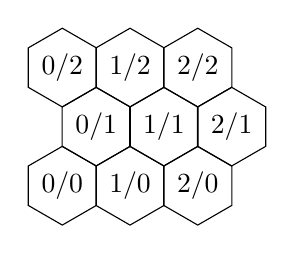
\begin{tikzpicture}
        \foreach \off / \x / \y in {0/0/0,0/1/0,0/2/0,0.43cm/0/1,0.43cm/1/1,0.43cm/2/1,0/0/2,0/1/2,0/2/2} {
            \draw ({\off + \x*0.86cm},{0.75cm * \y}) -- ++(30:0.5cm)
              \foreach \r in {90,150,210,270,330} { -- ++(\r:0.5cm) }
              -- cycle;
          \draw ({\off + \x*0.86cm},{0.75cm * \y + 0.5cm}) node {\x/\y};
        };
    \end{tikzpicture}
    \caption{hexagonal}
    \label{fig:coord-hex}
    \end{subfigure}

    \begin{subfigure}{1\linewidth}
        \centering
    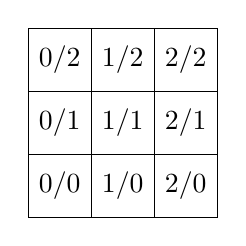
\begin{tikzpicture}
        \foreach \off / \x / \y in {0/0/0,0/1/0,0/2/0,0.43cm/0/1,0.43cm/1/1,0.43cm/2/1,0/0/2,0/1/2,0/2/2} {
            \draw ({0.8cm * \x},{0.8cm * \y})
              -- ++({0.8cm},{0})
              -- ++({0},{0.8cm})
              -- ++({-0.8cm},{0})
              -- cycle;
          \draw ({\x*0.8cm + 0.4cm},{0.8cm * \y + 0.4cm}) node {\x/\y};
        };
    \end{tikzpicture}
    \caption{rectangular}
    \label{fig:coord-rect}
    \end{subfigure}
    \caption{Coordinate system and layout}
    \label{fig:coord}
\end{figure}

To abstract the grid neighbourhood, geometric layout and rendering from the actual 3d \lstinline!Unit! array
representation a new interface has been introduced. The interface \lstinline!GridHelper! is the base abstraction
to be able to calculate shapes, center of the shapes and the grid neighbours.

\bibliography{ref}
\bibliographystyle{plain}

\end{document}
